%%%%%%%%%%%%%%%%%%%%%%%%%%%%%%%%%%%%%%%%%
%%% HYPERRIDE Reporting Template
%%%%%%%%%%%%%%%%%%%%%%%%%%%%%%%%%%%%%%%%%

\documentclass[letterpaper,12pt]{report}
\usepackage[pass]{geometry}
\usepackage{xcolor}
\usepackage{hyperride}		% HYPERRIDE specific definitions and styles  
\usepackage[utf8]{inputenc}	% UTF8 package
\usepackage[T1]{fontenc}
\usepackage{textcomp}		% common special chars
\usepackage{amsmath}		% math formula
\usepackage{fancybox}
\usepackage{anyfontsize}	% fonts
\usepackage{lipsum}
\usepackage{float}
\usepackage[normalem]{ulem}
\usepackage{cleveref}
\usepackage[printonlyused]{acronym}
\hypersetup{
	pdftitle={Beacon Network Security Labs: Middlebox Amplification Attack Lab},
	pdfauthor={[Jordan Whyte, Gaby Dagher]},
	pdfkeywords={Beacon Labs, Middlebox, TCP Amplification, Network Security},
}
\usepackage{subfigure}
\usepackage{graphicx}
\usepackage{xcolor}
\usepackage{soul}
\sethlcolor{lightgray}
\usepackage[export]{adjustbox}
\usepackage{mdframed}
\usepackage{pdfpages}
\usepackage{comment}
\usepackage{multirow,array}
\def\todo#1{{\color{hyperridered}\textbf{TODO:} ``#1''}}
\def\hyperride{HYPERRIDE}
\definecolor{lightblue}{rgb}{0.87, 0.94, 1}
\graphicspath{ {graphics/} }

%%%%%%%%%%%%%%%%%%%%%%%%%%%%%%%%%%%%%%%%%
%%% Definitions
%%%%%%%%%%%%%%%%%%%%%%%%%%%%%%%%%%%%%%%%%

\begin{document}


\includepdf[pages=1]{./graphics/2FP.pdf}

\mdfdefinestyle{code}{%
    linecolor=black,
    outerlinewidth=2pt,
    %roundcorner=20pt,
    innertopmargin=4pt,
    innerbottommargin=4pt,
    innerrightmargin=4pt,
    innerleftmargin=4pt,
        leftmargin = 4pt,
        rightmargin = 4pt
    backgroundcolor=black!10
    }

\setcounter{tocdepth}{4}
\setcounter{secnumdepth}{4}

%%%%%%%%%%%%%%%%%%%%%%%%%%%%%%%%%%%%%%%%%
%%% URL style same as regular text
%%%%%%%%%%%%%%%%%%%%%%%%%%%%%%%%%%%%%%%%%
	
\urlstyle{same}

%%%%%%%%%%%%%%%%%%%%%%%%%%%%%%%%%%%%%%%%%
%%% Deliverable Information
%%%%%%%%%%%%%%%%%%%%%%%%%%%%%%%%%%%%%%%%%

% Project Meta Information
\ProjectFullTitle{Beacon Network Security Labs: Middlebox Amplification Attack Lab}
\ProjectAcronym{HYPERRIDE}
\ProjectRefNo{957788}

% Report Number, use either "1", "2", or "3" for the corresponding reporting period
\delivNumber{0}

% Period covered by the report
\delivFrom{dd/mm/yyyy}
\delivTo{dd/mm/yyyy}

% Report Responsible Partner
\delivResponsible{AIT Austrian Institute of Technology (AIT)} 

% Report Version, Contractual and Actual Date, Dissemination Level, Type
\delivVersion{vn.n}
\ContractualDate{dd/mm/yyyy}
\ActualDate{dd/mm/yyyy}

% List of Main Authors (usually from the responsible partner)
\delivAuthor{[Jordan Whyte, Gaby Dagher]}

% List of Co-Authors (all other co-authors should be listed here)
\delivFPAuthor{[]}

% Report Status
\delivStatus{d} %% d = draft, f = final, s = submitted

%%%%%%%%%%%%%%%%%%%%%%%%%%%%%%%%%%%%%%%%%
%%% Change Log
%%%%%%%%%%%%%%%%%%%%%%%%%%%%%%%%%%%%%%%%%

\istChange{dd/mm/yyyy}{v1.0}{Name (Partner short name)}{Draft report template}
\istChange{}{}{}{}

%%%%%%%%%%%%%%%%%%%%%%%%%%%%%%%%%%%%%%%%%
%%% Cover Page
%%%%%%%%%%%%%%%%%%%%%%%%%%%%%%%%%%%%%%%%%

%\makecover

%%%%%%%%%%%%%%%%%%%%%%%%%%%%%%%%%%%%%%%%%
%%% Table of Contents
%%%%%%%%%%%%%%%%%%%%%%%%%%%%%%%%%%%%%%%%%

\clearpage
\fancypagestyle{plain}{}
\settableofcontents
\tableofcontents
\clearpage

%%%%%%%%%%%%%%%%%%%%%%%%%%%%%%%%%%%%%%%%%
%%% Overview
%%%%%%%%%%%%%%%%%%%%%%%%%%%%%%%%%%%%%%%%%
\newpage
\section*{Overview}\label{sec:work-carried-out}
\addcontentsline{toc}{section}{Overview}

\textbf{Objective}

Further understand the 5 types of reflection-based attacks performed in this lab using TCP instead of UDP.

\textbf{TCP-based Reflection Attacks}

Reflection amplification attacks were thought to only be possible through UDP because there was no three-way handshake that took place. However, this type of attack was found to be possible through TCP in 2021 due to the existence of middleboxes, such as firewalls, that capture traffic before the server can respond to it.

Without a three-way handshake, the server should just drop unrecognized packets. Instead, the middlebox attempts to respond to the request before the server sees it. These middleboxes are often firewalls that attempt to respond to forbidden requests with blocked pages, but their response can be large, even up to an infinite number of packets, relative to the one initial request. These attacks seek to exploit that vulnerability.

\textbf{Packet Schemes and Amplification Factors}

Different packet schemes produced different responses from the middleboxes resulting in large or small amplification factors as seen in Figure~\ref{fig:Packet_Type_Response} below.

\begin{figure}[!h]
    \centering
    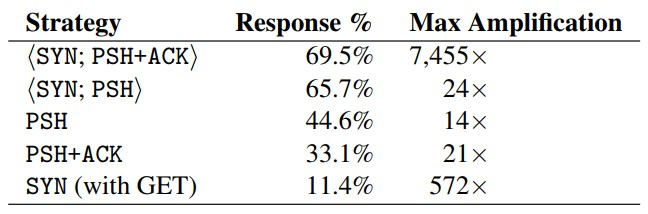
\includegraphics[width=0.7\columnwidth]{graphics/packet_type_response.jpg}
    \caption{Packet Type Response}
    \label{fig:Packet_Type_Response}
\end{figure}

Moreover, the type of forbidden page that was requested produced a different response as demonstrated in Figure~\ref{fig:webpage_response}.

\begin{figure}[!h]
    \centering
    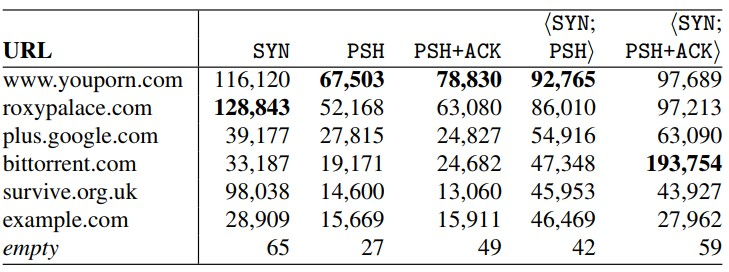
\includegraphics[width=0.7\columnwidth]{graphics/url_IP_address.jpg}
    \caption{Number of IP addresses with amplification factor over 100x for each combination of target URL and packet sequence. Bolded is the maximum value for each sequence.}
    \label{fig:webpage_response}
\end{figure}

\textbf{Types of Middlebox Amplification}

There are five types of amplifications that can be produced through this method of attack:

\begin{enumerate}
    \item \textit{Destination Reflection}
    \begin{enumerate}
        \item Direct response of static size from the destination.
        \item Example: 2Mb response to a 1Mb ping.
    \end{enumerate}
    \item \textit{Middlebox Reflection}
    \begin{enumerate}
        \item Initial ping of packet size 1Mb receiving a block page of static size 10Mb (10x Amplification).
    \end{enumerate}
    \item \textit{Destination and Middlebox Reflection}
    \begin{enumerate}
        \item A combination of the first two methods: A static size middlebox and destination response.
    \end{enumerate}
    \item \textit{Routing Loop Reflection}
    \begin{enumerate}
        \item All routers that a packet travels through will produce a middlebox response and loop back to each other.
        \item Amplification increases by the number of times routers trigger the middlebox.
    \end{enumerate}
    \item \textit{Victim-sustained Reflection}
    \begin{enumerate}
        \item Packets sent to the victim computer are responded to, prompting another response from the destination.
        \item Possible to produce an infinite amplification factor.
    \end{enumerate}
\end{enumerate}

\textbf{Resources}

Reading the following paper is not mandatory but will provide a deeper understanding of this attack and its outcomes:

\textit{Paper detailing the attack:}
\url{https://www.usenix.org/system/files/sec21-bock.pdf} $^\text{[\citeauthor{Bock:2021}]}$

%%%%%%%%%%%%%%%%%%%%%%%%%%%%%%%%%%%%%%%%%
%%% Setup
%%%%%%%%%%%%%%%%%%%%%%%%%%%%%%%%%%%%%%%%%

\section*{Setup}\label{sec:Setup}
\addcontentsline{toc}{section}{Setup}

\subsection*{Checking if Java is Installed}\label{sec:Checking-if-Java-is-Installed}
\addcontentsline{toc}{subsection}{Checking if Java is Installed}

\bigskip

\begin{mdframed}[backgroundcolor=black!10,style=code,nobreak=true,align=center,userdefinedwidth=14cm]
    \$ java -{}-version
\end{mdframed}

As long as your Java version is Java 11 or newer, you will be able to run this lab successfully.

If you don't have Java, please visit the following link to download a Java installer for your operating system. If any issues are encountered, simply Google "Java install guide for <operating system>" where <operating system> is the operating system you are using.

\url{https://www.java.com/en/}

\subsection*{Compiling TCPAmplificationAttackLab}\label{sec:Compiling-TCPAmplificationAttackLab}
\addcontentsline{toc}{subsection}{Compiling TCPAmplificationAttackLab}

The \href{https://drive.google.com/file/d/14CoMaemmpK28jwWu3SaxBnkj2ScTdDmq/view?usp=drive_link}{program} for this lab will be in the \href{https://drive.google.com/drive/folders/1eKRoJG2hiRVtAQwjhZOw5exEAlkPk16H?usp=drive_link}{Lab 2 folder}.

Once you have completed the first task of the lab, you can continue on to the program using the directions below. The lab is an entirely self contained java program.

To compile and run the Java program, execute the following two commands:

\bigskip

\begin{mdframed}[backgroundcolor=black!10,style=code,nobreak=true,align=center,userdefinedwidth=14cm]
    \$ javac TCPAmplificationAttackLab.java\\
    \$ java TCPAmplificationAttackLab
\end{mdframed}

The TCPAmplificationAttackLab program should assist in the completetion of Task Set 2.

%%%%%%%%%%%%%%%%%%%%%%%%%%%%%%%%%%%%%%%%%
%%% Lab Task Set 1: Amplification Types
%%%%%%%%%%%%%%%%%%%%%%%%%%%%%%%%%%%%%%%%%

\section*{Task Set 1: Amplification Types}\label{sec:Task-Set-Amplification}
\addcontentsline{toc}{section}{Task Set 1: Amplification Types}

\textbf{Objective}

Acquire the ability to accurately identify the amplification type produced by an attack.

\subsection*{Task 1.1: Identify the Amplification Type}\label{sec:Task-1.1-Identify-the-Amplification-Type}
\addcontentsline{toc}{subsection}{Task 1.1: Identify the Amplification Type}

Based on the descriptions of the different types of amplifications provided in the Overview section, indicate which type of amplification each diagram below illustrates.

\colorbox{lightblue}{%
\parbox{\dimexpr\linewidth-2\fboxsep}{%
\textbf{Action}

1.1.1 - Describe the diagrams provided below and match each diagram to its corresponding type of amplification.
   }%
}%

\begin{figure}[!h]
    \centering
    \begin{minipage}{0.49\textwidth}
        \centering
        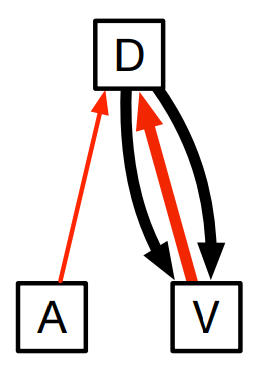
\includegraphics[width=.5\textwidth]{Victim_sustained_reflection.png}
        
        \label{fig:Victim_sustained_reflection}
    \end{minipage}
    \hfill
    \begin{minipage}{0.49\textwidth}
        \centering
        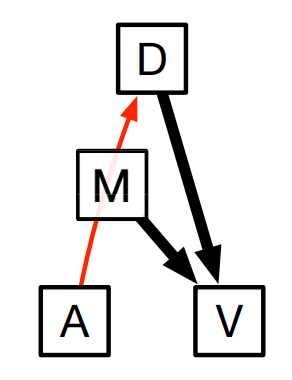
\includegraphics[width=.5\textwidth]{Destination_middlebox_reflection.png}
        
        \label{fig:Destination_middlebox_reflection}
    \end{minipage}
\end{figure}

\bigskip

\bigskip

\begin{figure}[!h]
    \centering
    \begin{minipage}{0.49\textwidth}
        \centering
        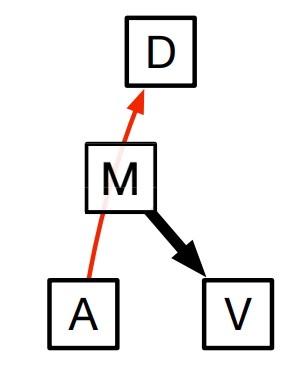
\includegraphics[width=.5\textwidth]{Middlebox_reflection.png}
        
        \label{fig:Middlebox_reflection}
    \end{minipage}
    \hfill
    \begin{minipage}{0.49\textwidth}
        \centering
        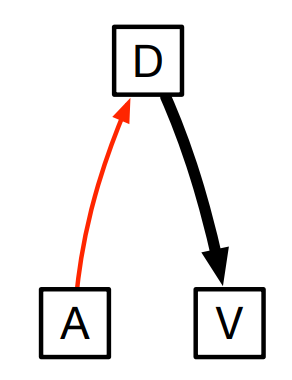
\includegraphics[width=.5\textwidth]{Destination_reflection.png}
       
        \label{fig:Destination_reflection}
    \end{minipage}
\end{figure}

\bigskip

\bigskip

\begin{figure}[!h]
    \centering
    \begin{minipage}{0.49\textwidth}
        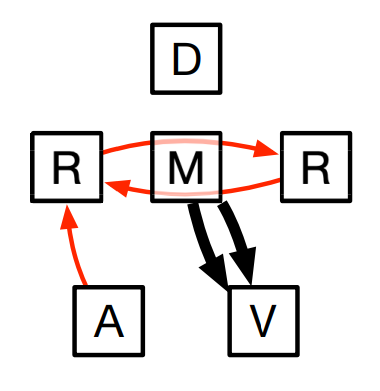
\includegraphics[width=0.6\textwidth]{Routing_loop.png}
    
    \label{fig:Middlebox_reflection}
    \end{minipage}
    \hfill
    \begin{minipage}{0.49\textwidth}
        \centering
            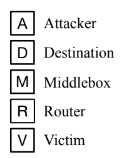
\includegraphics[width=.5\textwidth]{graphics/ADMRV.jpg}
       
        \label{fig:Destination_reflection}
    \end{minipage}
\end{figure}

%%%%%%%%%%%%%%%%%%%%%%%%%%%%%%%%%%%%%%%%%
%%% Lab Task Set 2: MiddleBox Amplification
%%%%%%%%%%%%%%%%%%%%%%%%%%%%%%%%%%%%%%%%%

\section*{Task Set 2: MiddleBox Amplification}\label{sec:Task-2}
\addcontentsline{toc}{section}{Task Set 2: MiddleBox Amplification}

\textbf{Objective}

Classify IP addresses depending on what type of reflection was produced.

\bigskip

This program will not actually send out packets to these IP addresses. The program is simply a simulation of the responses that would likely occur when this attack is executed properly.

\subsection*{Task 2.1: Running the Program}\label{sec:Task-2.1-Running-the-Program}
\addcontentsline{toc}{subsection}{Task 2.1: Running the Program}

Use the guide in the Setup section to get the program started. Figure~\ref{fig:program_start} shows the starting screen when running the program, and Figure~\ref{fig:packet_creation} shows how packets can be altered before being sent out.

\begin{figure}[!h]
    \centering
    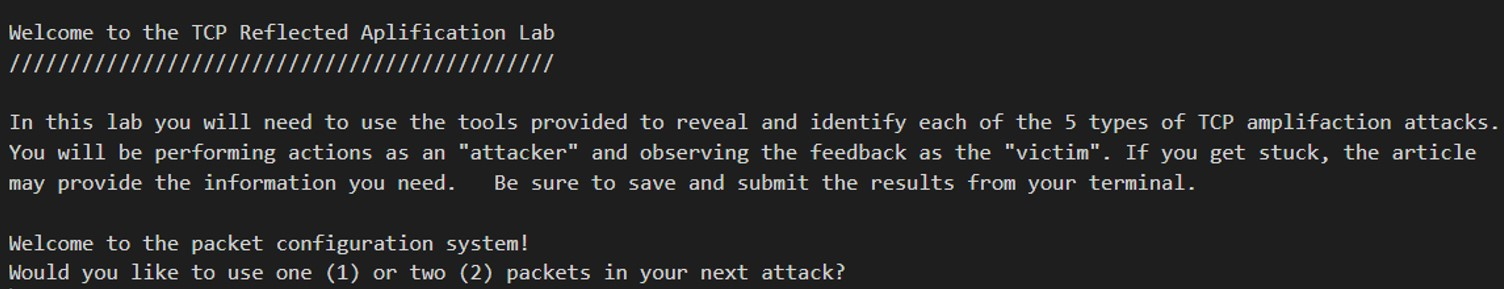
\includegraphics[width=1\columnwidth]{graphics/program_start_screen.jpg}
    \caption{Program start screen}
    \label{fig:program_start}
\end{figure}

\begin{figure}[!h]
    \centering
    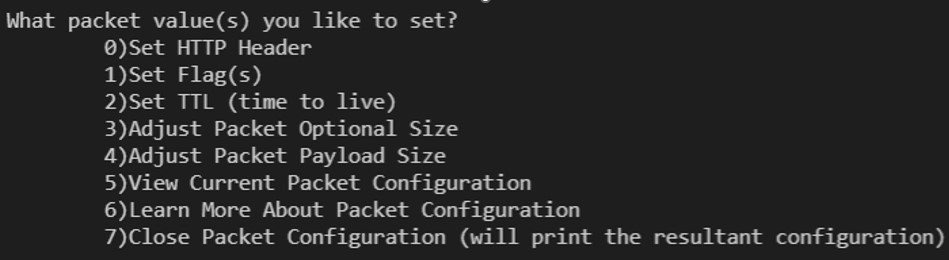
\includegraphics[width=1\columnwidth]{graphics/packet_creation_module.jpg}
    \caption{Packet creation module with different options for changing that packets that will be sent.}
    \label{fig:packet_creation}
\end{figure}

Within the program, you should first craft what kind of packet you want to send out. This requires setting the HTTP header, flags, time to live (TTL), and adjusting the size of the packet and payload to be sent. Using the crafted packet, you can then perform a wide attack, targeted attack, or a traceroute.

If you are unsure of what flags or header to use, hints can be found in Figures~\ref{fig:Packet_Type_Response} and~\ref{fig:webpage_response} in the Overview section.

\colorbox{lightblue}{%
\parbox{\dimexpr\linewidth-2\fboxsep}{%
\textbf{Action}

2.1.1 - Craft the type of packet you want to send out within the program.
    }%
}%

\bigskip

\subsection*{Task 2.2: Interacting with the Program}\label{sec:Task-2.2-Interacting-with-the-Program}
\addcontentsline{toc}{subsection}{Task 2.2: Interacting with the Program}

A Wide attack will send your packet to all IPs and show how many packets were sent in response. A Targeted attack will allow you to send your packet to one IP and observe how many packets are sent in response.

A traceroute will show the path a packet takes on the way to its destination. This will be useful in identifying what kind of amplification took place. \textbf{Some of the traceroutes will look identical, but based on the number of packets in response you should be able to identify what type of reflection it is, if there is reflection at all. }

\begin{figure}[!h]
    \centering
    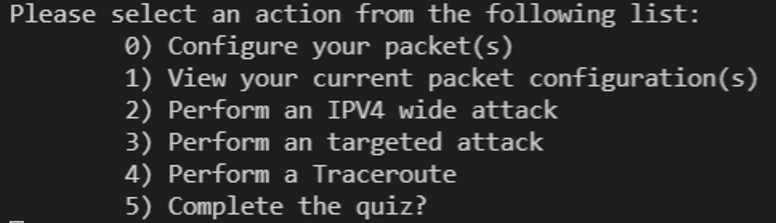
\includegraphics[width=1\columnwidth]{graphics/all_actions.jpg}
    \caption{All actions that can be performed in the program.}
    \label{fig:program_action_list}
\end{figure}

All tools listed in Figure~\ref{fig:program_action_list} are required to complete the lab with full points.

The following table shows everything that needs to be identified for the quiz.

\begin{center}
    \begin{tabular}{ |p{0.7\linewidth}|c|c| } 
         \hline
         \textbf{Quiz Question} & \textbf{Point Value} & \textbf{Total} \\
         \hline
         Which IPs produced amplification? (5x) & 8 & 40 \\ 
         \hline
         Which type of amplification is at each IP? (5x) & 5 & 25 \\ 
         \hline
         Destination response size & 5 & 5\\
         \hline
         Middlebox response size (2x) & 5 & 10\\
         \hline
         Number of routers in routing loop & 10 & 10\\
         \hline
         How many packets did the victim send in the victim-sustained attack? & 10 & 10\\
         \hline
    \end{tabular}
\end{center}

Keep track of these things as you work through the program. The quiz will ask you these questions and you can gain points for each. (\textit{Hint for the final question:} Assume the victim sent one packet to the server in response to each server packet)

\textit{Remember, not all combinations of packets will result in all attacks being performed. You may need to reconfigure the packet(s) in order to find all of the attacks.}

Each question will have a set number of attempts in case you mistype your answer. Additionally, you can run the program again to generate new IPs for each amplification and attempt to gain a better score.

\colorbox{lightblue}{%
\parbox{\dimexpr\linewidth-2\fboxsep}{%
\textbf{Action}

2.2.1 - Run the program as explained in the setup section of this document.\\ 
2.2.2 - Complete the quiz.\\
2.2.3 - Save a screenshot of your console's output to display your final score in your lab report.\\ 
    }%
}%

%%%%%%%%%%%%%%%%%%%%%%%%%%%%%%%%%%%%%%%%%
%%% Lab Task Set 3: Game Theory
%%%%%%%%%%%%%%%%%%%%%%%%%%%%%%%%%%%%%%%%%

\section*{Task Set 3: Bayesian Nash Equilibrium }\label{sec:Task-Set-3}
\addcontentsline{toc}{section}{Task Set 3: Bayesian Nash Equilibrium}

\textbf{Objective}

Further comprehend the Bayesian Nash Equilibrium through analysis of a Game Theory table and application of the concept to a hypothetical scenario.

\subsection*{Task 3.1: Understanding Bayesian Nash Equilibrium}\label{sec:Task-3.1-Understanding-Bayesian-Nash-Equilibrium}
\addcontentsline{toc}{subsection}{Task 3.1: Understanding Bayesian Nash Equilibrium}

Game theory can be applied to more than just a two party situation. Deciding which action should be taken when there is uncertainty of the other party can be solved with Bayesian Nash Equilibrium. Keep in mind, \textbf{Bayesian Nash equilibrium only works when no one has incentive to change their strategy based on prior beliefs of the other party}.

\bigskip

Bayesian Nash Equilibrium will be demonstrated on Table~\ref{Tab:game_theory_1}, then you will apply it to the made-up scenario following Table~\ref{Tab:game_theory_1}.

\begin{table}[ht]
    \setlength{\extrarowheight}{2pt}
    \begin{tabular}{cc|c|c|}
      & \multicolumn{1}{c}{} & \multicolumn{2}{c}{\color{red}Player 2}\\
      & \multicolumn{1}{c}{} & \multicolumn{2}{c}{\color{red}A-Type}\\
      & \multicolumn{1}{c}{} & \multicolumn{1}{c}{\color{red}Left}  & \multicolumn{1}{c}{\color{red}Right} \\\cline{3-4}
      \multirow{2}*{\color{blue}Player 1}  & \color{blue}Up & $\color{blue}(6,\color{red}2)$ & $\color{blue}(0,\color{red}4)$ \\\cline{3-4}
      & \color{blue}Down & $\color{blue}(5,\color{red}1)$ & $\color{blue}(-1,\color{red}4)$ \\\cline{3-4}
    \end{tabular}
    \begin{tabular}{cc|c|c|}
      & \multicolumn{1}{c}{} & \multicolumn{2}{c}{\color{red}Player 2}\\
      & \multicolumn{1}{c}{} & \multicolumn{2}{c}{\color{red}B-Type}\\
      & \multicolumn{1}{c}{} & \multicolumn{1}{c}{\color{red}Left}  & \multicolumn{1}{c}{\color{red}Right} \\\cline{3-4}
      \multirow{2}*{}  & \color{blue}Up & $\color{blue}(3,\color{red}4)$ & $\color{blue}(1,\color{red}0)$ \\\cline{3-4}
      & \color{blue}Down & $\color{blue}(4,\color{red}3)$ & $\color{blue}(2,\color{red}0)$ \\\cline{3-4}
    \end{tabular}
\caption{Game Theory Example}
\label{Tab:game_theory_1}
\end{table}

There is a chance that Player 1 will be either A-Type or B-Type. We will represent this with the variable $P$. There are still only two options for both players to choose but, Player 2 does not know what type Player 1 is. Furthermore, Player 1 can only see the table corresponding to their type while Player 2 can see both tables.

Player 2 must first see what the dominant strategy is for Player 1 in each scenario. This is quite simple though as with A-Type, Up strictly dominates Down, and for B-Type, Down strictly dominates Up. With this information, the table Player 2 is working with now looks like Table~\ref{Tab:game_theory_2}, located at the top of the next page.

\begin{table}[!bt]
    \setlength{\extrarowheight}{2pt}
    \begin{tabular}{cc|c|c|}
      & \multicolumn{1}{c}{} & \multicolumn{2}{c}{\color{red}Player 2}\\
      & \multicolumn{1}{c}{} & \multicolumn{2}{c}{\color{red}A-Type}\\
      & \multicolumn{1}{c}{} & \multicolumn{1}{c}{\color{red}Left}  & \multicolumn{1}{c}{\color{red}Right} \\\cline{3-4}
      \multirow{2}*{\color{blue}Player 1}  & \color{blue}Up & $\color{blue}(6,\color{red}2)$ & $\color{blue}(0,\color{red}4)$ \\\cline{3-4}
      & \color{blue}Down &  &  \\\cline{3-4}
    \end{tabular}
    \begin{tabular}{cc|c|c|}
      & \multicolumn{1}{c}{} & \multicolumn{2}{c}{\color{red}Player 2}\\
      & \multicolumn{1}{c}{} & \multicolumn{2}{c}{\color{red}B-Type}\\
      & \multicolumn{1}{c}{} & \multicolumn{1}{c}{\color{red}Left}  & \multicolumn{1}{c}{\color{red}Right} \\\cline{3-4}
      \multirow{2}*{}  & \color{blue}Up &  &  \\\cline{3-4}
      & \color{blue}Down & $\color{blue}(4,\color{red}3)$ & $\color{blue}(2,\color{red}0)$ \\\cline{3-4}
    \end{tabular}
\caption{Game Theory Example}
\label{Tab:game_theory_2}
\end{table}

\bigskip

Next we must calculate the utility of each action. What can Player 2 gain if they were to play left or right?

Remember that P is the probability of Player 1 being an A-Type. Thus, $1-P$ is the probability of Player 1 being a B-Type. To calculate the utility of Player 2 playing left, we take the utility from choosing left on both types times the probability of being that type. The same symbolic calculation was done to calculate the utility of Player 2 playing right.

$$\textbf{LEFT: } 2P + 3(1-P)$$
$$\textbf{RIGHT: }  4P + 0(1-P)$$

By solving an inequality we can see when Player 2 should play left or right.

$$ 2P + 3(1-P) > 4P + 0(1-P) $$
$$ 2P + 3 - 3P  > 4P $$
$$ 3 - P > 4P $$
$$ 3 > 5P $$
$$ \frac{3}{5} > P $$

So when P is less than $\frac{3}{5}$, Player 2 should play left, but when $P$ is greater than or equal to $\frac{3}{5}$ they should play right.

\subsection*{Task 3.2: Applying Bayesian Nash Equilibrium with an Exercise}\label{sec:Task-3.2-Applying-Bayesian-Nash-Equilibrium-With-an-Exercise}
\addcontentsline{toc}{subsection}{Task 3.2: Applying Bayesian Nash Equilibrium with an Exercise}

Use the concepts learned in Task 3.1 to answer the questions in Task 3.2.

\begin{table}[ht]
    \setlength{\extrarowheight}{2pt}
    \begin{tabular}{cc|c|c|}
      & \multicolumn{1}{c}{} & \multicolumn{2}{c}{\color{red}Attacker}\\
      & \multicolumn{1}{c}{} & \multicolumn{2}{c}{\color{red}A-Type}\\
      & \multicolumn{1}{c}{} & \multicolumn{1}{c}{\color{red}New Attack}  & \multicolumn{1}{c}{\color{red}Old Attack} \\\cline{3-4}
      \multirow{2}*{\color{blue}Server}  & \color{blue}No one watching server & $\color{blue}(1,\color{red}5)$ & $\color{blue}(2,\color{red}3)$ \\\cline{3-4}
      & \color{blue}Someone watching server & $\color{blue}(3,\color{red}4)$ & $\color{blue}(2,\color{red}2)$ \\\cline{3-4}
    \end{tabular}
    \begin{tabular}{cc|c|c|}
      & \multicolumn{1}{c}{} & \multicolumn{2}{c}{\color{red}Attacker}\\
      & \multicolumn{1}{c}{} & \multicolumn{2}{c}{\color{red}B-Type}\\
      & \multicolumn{1}{c}{} & \multicolumn{1}{c}{\color{red}New Attack}  & \multicolumn{1}{c}{\color{red}Old Attack} \\\cline{3-4}
      \multirow{2}*{\color{blue}Server}  & \color{blue}No one watching server & $\color{blue}(2,\color{red}2)$ & $\color{blue}(3,\color{red}3)$ \\\cline{3-4}
      &\color{blue}Someone watching server & $\color{blue}(1,\color{red}1)$ & $\color{blue}(2,\color{red}1)$ \\\cline{3-4}
    \end{tabular}
\caption{Game Theory Task}
\label{Tab:game_theory_3}
\end{table}

Let's say that there are two countries that you want to use this new attack on. Country 1 is the primary target and Country 2 is an ally. The server you are attacking is a server positioned on the shared border of the two countries so, there is a chance that it could be administered by either.

You could either use an old attack so that they are unaware of the new vulnerability, but it may be less effective, or, you could use this new attack with which you could do more damage, but be unable to use it in the future as the vulnerability was patched.

The A-Type server is Country One (the primary target), and B-Type is Country Two (the ally). Using these tables, answer the following questions:

\colorbox{lightblue}{%
\parbox{\dimexpr\linewidth-2\fboxsep}{%
\textbf{Action}

3.2.1 - Write your inequality.\\ 
3.2.2 - Solve your inequality then Answer the following questions. Show your work in your submission.\\
    }%
}%

\bigskip

\begin{mdframed}[backgroundcolor=black!10,style=code,nobreak=true,align=center,userdefinedwidth=14cm]
    Which attack should you use if there is a $\frac{1}{2}$ chance the server is owned by country one?

    Which attack should you use if there is a $\frac{1}{3}$ chance the server is owned by country one?

    Which attack should you use if there is a $\frac{1}{4}$ chance the server is owned by country one?
\end{mdframed}

%%%%%%%%%%%%%%%%%%%%%%%%%%%%%%%%%%%%%%%%%
%%% Submission
%%%%%%%%%%%%%%%%%%%%%%%%%%%%%%%%%%%%%%%%%

\section*{Submission}\label{sec:Submission}
\addcontentsline{toc}{section}{Submission}

Include all the deliverables in the lab report, and submit your completed lab report using the provided \href{https://docs.google.com/document/d/1f_rB22EzL8aezExZ7jYFARnuy5xuhcwC/edit?usp=sharing&ouid=113481593569562690929&rtpof=true&sd=true}{lab report template}. 

Demonstrate your thinking for each task through text and images as needed. For lab task 3, show what $P$ should be equal to and answers to each question. Submit the completed lab report to your instructor as specified.

%%%%%%%%%%%%%%%%%%%%%%%%%%%%%%%%%%%%%%%%%
%%% Summary
%%%%%%%%%%%%%%%%%%%%%%%%%%%%%%%%%%%%%%%%%

\section*{Summary}\label{sec:Sumarry}
\addcontentsline{toc}{section}{Summary}

Reflection based attacks have been common over UDP but, this is the first time they have been possible over TCP. This lab has taught you about the kinds of middlebox reflections and how to identify them.

TCP reflection based attacks are a large vulnerability that has major ramifications across many nations who have a high amount of censorship. To learn the extent of this vulnerability, the paper$^\text{[\citeauthor{Bock:2021}]}$ is listed in both the Overview and References section.

\bibliography{References}
\bibliographystyle{plain}

\end{document}

%%%%%%%%%%%%%%%%%%%%%%%%%%%%%%%%%%%%%%%%%